\section{Приклади}

\vspace{-\baselineskip}

\subsection{Одна з перших робіт з оцифровування дошки}

У 2004 році інженери з Microsoft Research \textit{Zhengyou Zhang}
та \textit{Li-wei He} представили свій алгоритм по скануванню написів
білої дошки.

В їхній роботі \cite{zhang:2004} обробляються фотографії білої дошки. Локалізується область
дошки, вирівнюється у прямокутну форму і бінаризуються написи без втрати
кольору.(рис. \ref{fig:zhang:2004}).
\begin{figure}[h]
  \centering
  \begin{subfigure}[b]{0.4\textwidth}
    \centering
    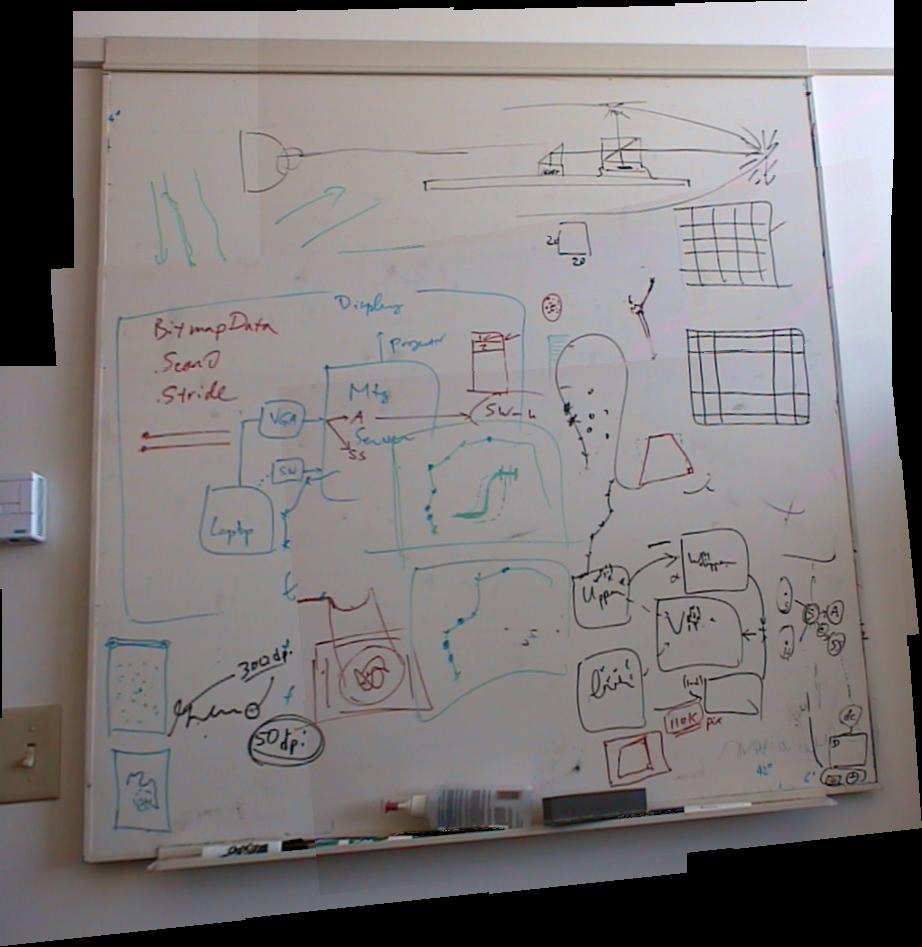
\includegraphics[width=\textwidth]{images/zhang_2004_1}
  \end{subfigure}
  \begin{subfigure}[b]{0.3\textwidth}
    \centering
    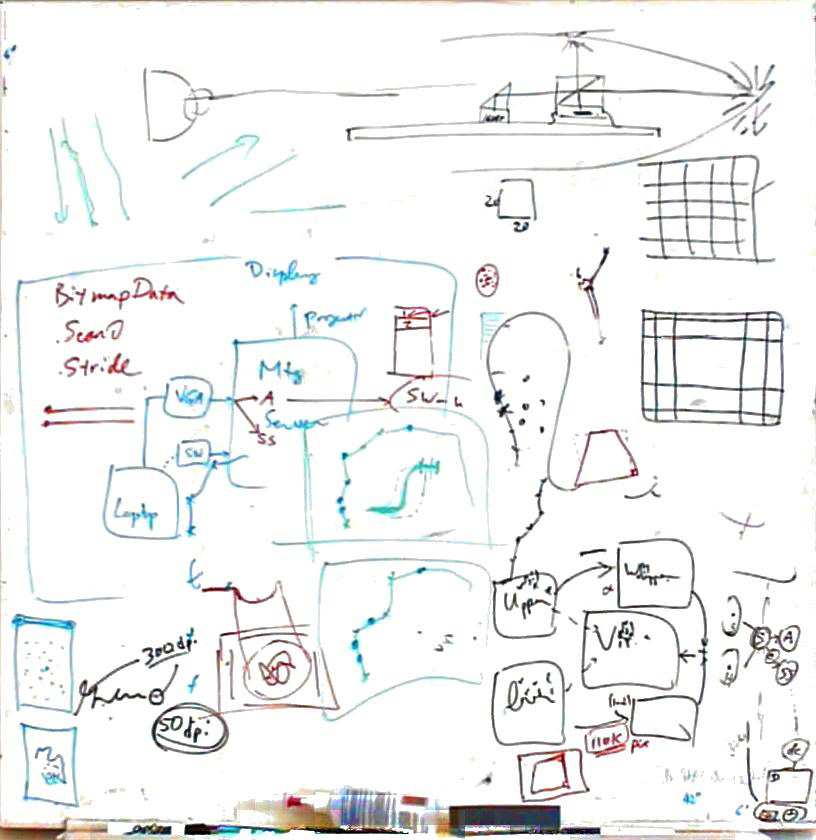
\includegraphics[width=\textwidth]{images/zhang_2004_2}
  \end{subfigure}
  \label{fig:zhang:2004}
  \caption{Демонстрація роботи алгоритму інженерів з Microsoft}
\end{figure}

Також автори реалізували склейку зображень дошки зроблених з різних
перспектив за допомогою гомографії. Гарна якість оцифрування дошки
досягається насамперед тим, що вона має білий колір, що в свою чергу
накладає обмеження для використання технології з дошками зеленого чи
чорного кольорів.
У наступній свої роботі \cite{zhang:2007} ціж самі автори побудували
систему, яка в реальному часі обробляє відеозапис, видаляє людину біля 
дошки за допомогою часової медіани, але в даному випадку немає 
панорамного склеювання знімків. Головна ідея роботи була зробити 
програму для телеконференсій.

\subsection{Автоматичне сканування дошки}

Автори даної роботи \cite{wienecke} створили програму яка переводить написи на білій 
дошці у цифрові. Вони реалізували локалізацію тексту та подальшу 
його обробку. Дана технологія не передбачає перекривання викладачем написів
або дошку іншого кольору відмінного від білого.

\begin{figure}[h]
  \centering
  \begin{subfigure}[b]{0.3\textwidth}
    \centering
    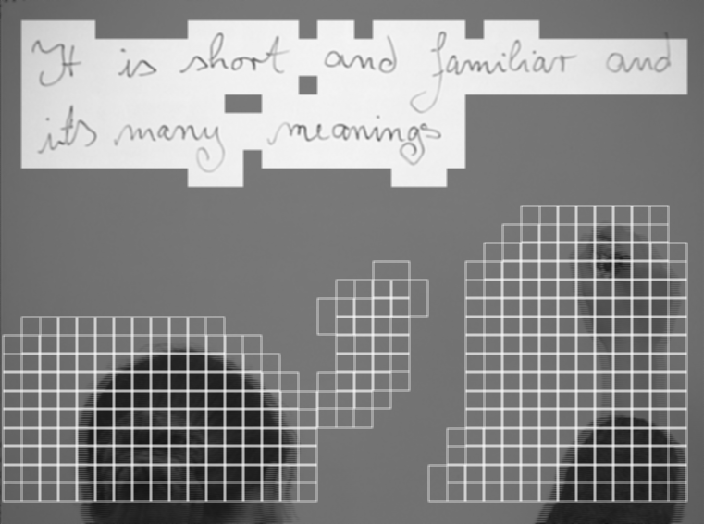
\includegraphics[width=\textwidth]{images/wienecke_1}
  \end{subfigure}
  \begin{subfigure}[b]{0.3\textwidth}
    \centering
    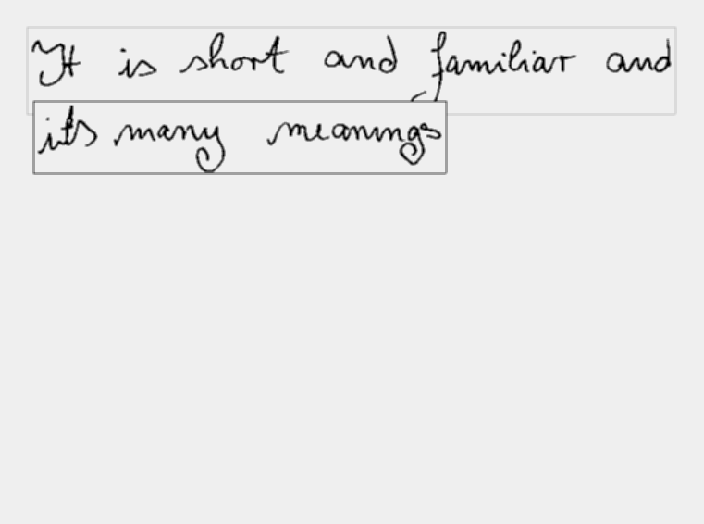
\includegraphics[width=\textwidth]{images/wienecke_2}
  \end{subfigure}
  \label{fig:wienecke}
  \caption{Демонстрація роботи сканування дошки}
\end{figure}

Можна помітити, що як і в попередній роботі гарна якість виокремлення написів
досягається тим що дошка білого кольору.

\subsection{Відстежування об'єкту та віднімання фону від Стенфорду}

У 2012 році науковці зі Стенфордського університету \textit{Alex Gonzalez, 
Bongsoo Suh, Eun Soo Choi} представили технологію \cite{sah} локалізацію дошки
(навіть такої яка розділена на частини), відстеження викладача та його
подальше прибирання. Алгоритм також може працювати з різними кольрами
дошок. Для прибирання викладача і всіх рухомих об'єктів автори також 
використали тимчасову медіану.

Дана програма не працює в реальному часі, оскільки всі операції над кадрами
відео займають тривалий час, не кажучи вже, що відео перед обробкою 
піддають компресії.


\begin{figure}[h]
  \centering
  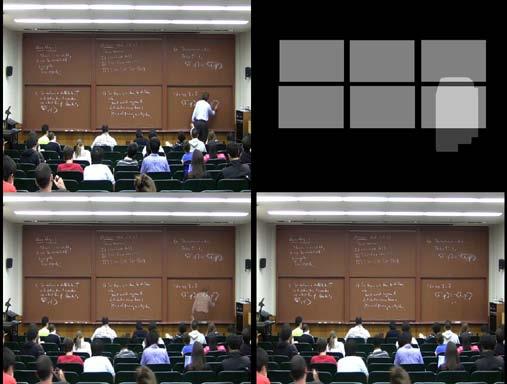
\includegraphics[width=0.5\textwidth]{images/sah}
  \caption{Приклад роботи авторів Стенфорду}
  \label{fig:sah}
\end{figure}


% Згодом ті ж автори розробили та використали у своїй роботі
% стохастичний алгоритм Ньютона \cite{blanz:vetter:2003},
% яким досягли реконструкції просторової конфігурації обличчя за 4.5 хвилини на
% Pentium 4, 2GHz.

% Важливою деталлю цієї породжувальної моделі є те,
% що кожна вершина різних моделей має однакове семантичне значення.
% Краї очей, рота, кінчик носу, підборіддя та інші точки
% знаходяться в однакових комірках масивів вершин моделей.
% BFM розмічена опорними точками з наборів Farkas та MPEG4 FDP
% (рис. \ref{fig:problems:feature-points}).
% Відповідність точок дає змогу створювати власні множини опорних точок.


% \subsection{Вітчизняна робота}

% У 2011 році Максим Тищенко,
% випускник Національного технічного университету України
% ``Київський політехнічний інститут'',
% працюючи у Міжнародному науково-навчальному центрі
% інформаційних технологій та систем над кандидатською дисертацією,
% запропонував та запатентував
% свій метод створення генеративної моделі обличчя та відновлення
% тривимірної поверхні обличчя за одним або кількома фото \cite{tyshchenko:2011}.
% Основні відмінності полягають у тому,
% що задачу співставлення відповідних точок різних моделей
% було представлено та розв'язано як супермодулярну
% задачу розмітки \cite{Lovasz1983},
% а нові моделі облич генеруються як зважене середнє.
% Проте було наявне спрощення: самозатінення не бралося до уваги,
% що дозволяло дуже швидко знаходити оптимальне освітлення
% за пласкою моделлю затінення методом найменших квадратів.

% \subsection{Сучасні роботи}

% На момент написання дисертації одними з новітніх робіт,
% де було використано модель Базельського університету,
% є методи відстеження обличчя \cite{Saito2016}
% та переносу виразу обличчя однієї людини іншій \cite{thies2016face}.
% Докладніше про них буде сказано в наступному підрозділі.
% Останньою відомою роботою
% є Large Scale 3D Morphable Models \cite{Booth:2017}~---~це
% генеративна модель обличчя, яка отримана з тривимірних знімків $10$ тисяч людей
% різної статі, віку та раси, що робить її дуже різноманітною та корисною
% (рис.~\ref{fig:problems:lsfm}).

% \begin{figure}[h]
%   \centering
%     \includegraphics[width=0.9\textwidth]{images/lsfm}
%   \caption{Приклади облич, що побудовані за допомогою LSFM}
%   \label{fig:problems:lsfm}
% \end{figure}
